\subsection{Quadcopter}
\subsubsection{Defination}
A quadcopter, also called a quadrotor helicopter, quadrocopter, quadrotor, is a multicopter that is lifted and propelled by four rotors.\cite{cite1}
\begin{figure}[h!]

  \centering
    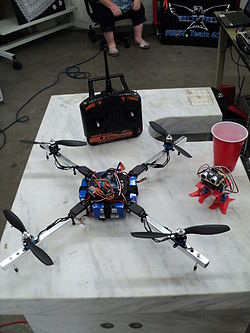
\includegraphics[width=0.3\textwidth]{../Pictures/250px-ReuseumMakerFaireQuadrotor.JPG}
    \caption{A Maker Faire quadcopter in Garden City, Idaho\cite{cite1}}\\
\end{figure}
\subsubsection{Flight Control}
\begin{figure}[h!]

  \centering
    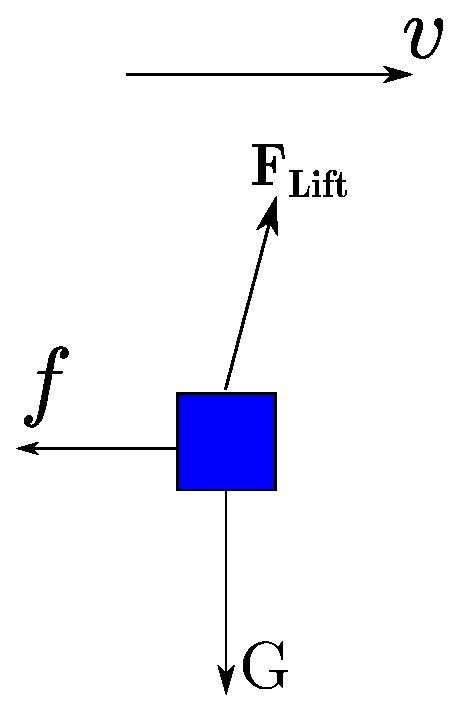
\includegraphics[width=0.3\textwidth]{../Pictures/flying.eps}
    \caption{The forces effected on the quadcopter while making stable movement.}\\
\end{figure}
%\newpage
\textbf{[ Hover ]}
\begin{figure}[H]

  \centering
    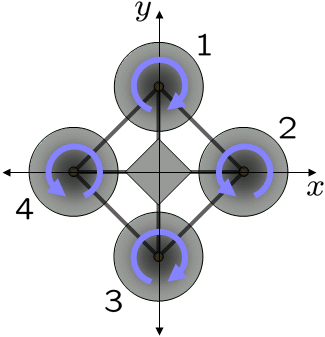
\includegraphics[width=0.3\textwidth]{../Pictures/Quadrotor_yaw_torque.png}
    \caption{The example model of quadcopter.}\\
\end{figure}


Each rotor produces both thrust and torque. If all the rotors are spinning at the same angular velocity, and as the example shows, with rotor 1,3 spinning clockwise and rotor 2,4 spinning counterclockwise, the angular acceleration on the yaw-axis will be zero.
This is the method to hovering.

\textbf{[ Yaw ]}\\
\begin{figure}[H]

  \centering
    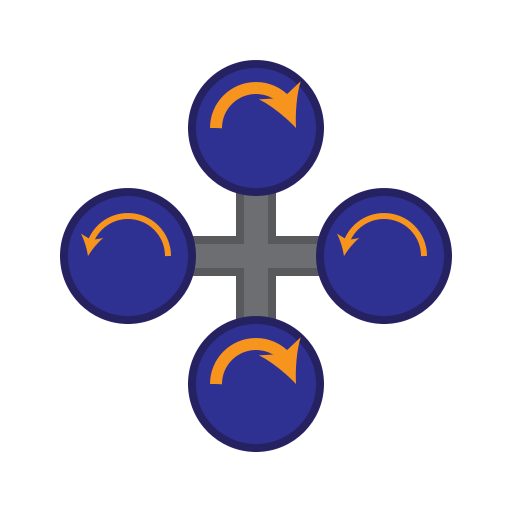
\includegraphics[width=0.3\textwidth]{../Pictures/yaw.png}
    \caption{Yaw control}
\end{figure}
The method of making yaw control can be done by adjusting the angular velocity of one pair of rotors.\\
\textbf{[ Pitch ]}\\
\begin{figure}[H]

  \centering
    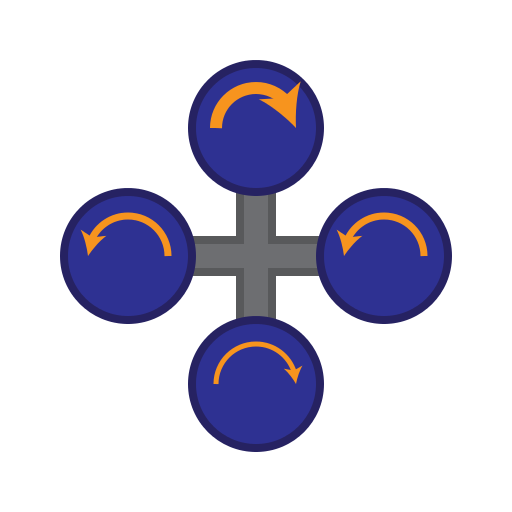
\includegraphics[width=0.3\textwidth]{../Pictures/pitch.png}
    \caption{Pitch control}
\end{figure}
The method of making pitch control can be done by increasing one rotor's spinning velocity and decreasing the opposite rotor's spinning velocity.\\
\textbf{[ Roll ]}\\
\begin{figure}[H]

  \centering
    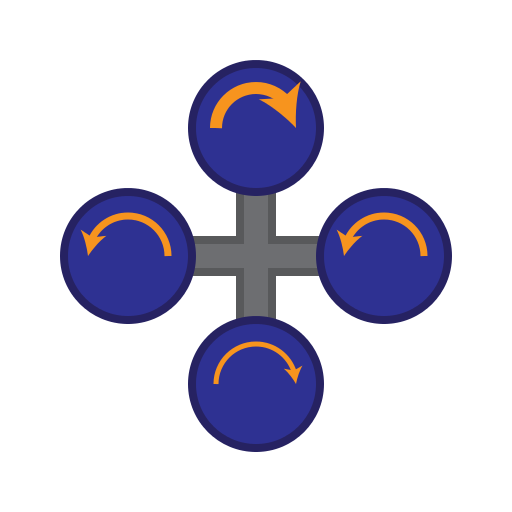
\includegraphics[width=0.3\textwidth, angle=90]{../Pictures/pitch.png}
    \caption{Roll control}
\end{figure}
The method of making roll control is similar to making pitch control.\\
It can be done by increasing one rotor's spinning velocity and decreasing the opposite rotor's spinning velocity.\\

\subsubsection{Design Principles}

This will probably remain an amateur project. Which means the time spent on this project will be relatively short. Therefore, we really want to keep things simple.

If there is an existing library that implemented a function we need, we can simply include the library in our project. Adoption of \emph{de facto} or \emph{de jure} standards make things not only \emph{simple}, but also \emph{easy to manage}.

After all, \emph{combination counts}.

\subsection{Computer Vision}
The basic computer vision system in this project will be \emph{OpenCV}\footnote{ OpenCV (Open Source Computer Vision Library) is a library of programming functions mainly aimed at real-time computer vision, developed by Intel, and now supported by Willow Garage and Itseez. \url{http://opencv.org}}.

There are several reasons for using \emph{OpenCV}:
\begin{itemize}
  \item Open source. \emph{OpenCV} is in BSD license. Therefore, our work can be perfectly legal, without any violation of IP laws.
  \item A large, active online community.
  \item The Intel background makes it reliable.
  \item Implemented in C++, the library is really fast.
\end{itemize}
Now, it is high time for discussing CV related issues.
\subsubsection{Quadcopter Identification}
The optimal choice, in this case, is a Quadcopter positioning system involves stereo visions and four colored table tennis balls on each Quadcopter.
The reason for that decision is fairly simple: \emph{simplicity}.
As seen in a youtube video, a research group did successfully implemented a tracking system which requires only mono-colored balls to locate quadcopters. \footnote{Something titled "Machine", "athletic", "Quadcopter". They used reflection markers as the tennis balls in this case.} While this is possible, it is also too complex for a small amateur team like ours to make it. However, multi-colored ball system can simplify the mechanism greatly. With limited time and computing power, this is the only logical choice.
